\documentclass[a4paper,10pt]{article}
\usepackage{fullpage}
\usepackage{float}
\usepackage[english]{babel}
\usepackage{graphicx,subfig,wrapfig}
\usepackage{amsmath,amsfonts,amsthm,amssymb}
\usepackage{fancyhdr,fancybox,color}
\usepackage{enumerate}
\usepackage[amssymb]{SIunits}             	% SI units package
\definecolor{MyBlue}{rgb}{0,0.3,0.6}
\usepackage[colorlinks=true,linkcolor=MyBlue,plainpages=false,citecolor=MyBlue,urlcolor=MyBlue]{hyperref}
\usepackage[all]{hypcap}   					%fixes the hyperref, such that links are anchored at the bottom of the images, not the top
\usepackage[url=false,
backend=bibtex,
style=authoryear-comp,
doi=true,
isbn=true,
backref=false,
dashed=false,
maxcitenames=2,
maxbibnames=99,
natbib=true]{biblatex}
\addbibresource{refrence.bib}
\nonfrenchspacing

\begin{document}

\noindent Chair: Physics of Fluids group
\begin{center}
	\begin{LARGE}
		Viscous dissipation controls drop impact: from thin films to deep pools 
	\end{LARGE}
\end{center}

\section*{Description}
Drops impacting a liquid layer can generate complex scenarios such as floating, bouncing, splashing, jetting, which have been extensively studied [1,2]. Among the different impact scenarios, a particularly intriguing phenomena is reported to occur at mild drop impact velocities [3,4]: floating or bouncing drops which never directly contact the underlying liquid layer. The reason for the drop repulsion is because of the lubrication pressure build-up in the draining thin gas layer between the droplet and the liquid layer which prevents the contact. A schematic diagram of a drop bouncing on a thin liquid film is shown in figure \ref{fig:bouncing_schematic}.\\

\begin{figure}[H]
\centering
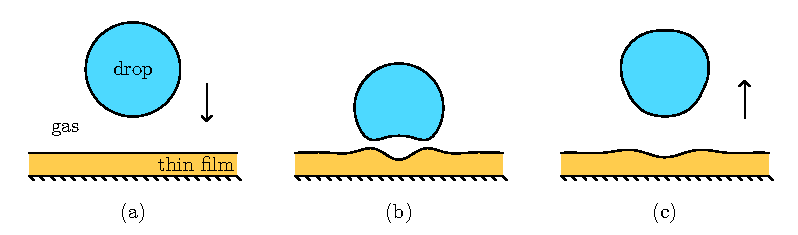
\includegraphics[width=0.75\textwidth]{drop_bounce_schematic.pdf}
\caption{Schematic diagram (not to scale) of a drop bouncing on a thin film in a surrounding gas environment. Three important stages in the bounce process are shown: (a) Initial (b) deformation and (c) relaxation stage.}
\label{fig:bouncing_schematic}
\end{figure}

In this work, we will perform experiments of a (oil/water) drop impacting a thin oil film in an ambient air environment. We plan to investigate the air layer and film deformations by varying three control parameters, namely the drop impact velocity $v_{w}$, film thickness $h_{f}$ and film viscosity $\eta_{f}$. The thin air layer deformations will be measured using Color Interferometry technique [5]. The thin film deformations will be measured using Digital Holographic Microscopy technique [6]. This measurements would give some valuable insight in the formation mechanism of the deformations which has not been previously studied. The synchronized recordings of the drop bouncing using a high speed camera and the oil surface deformation measured using Digital Holographic Microscopy setup are shown in the respective top and bottom rows in figure.\\

We will focus on the hydrodynamics of the process. In particular, we wish to understand various mechanisms through which the initial kinetic energy of the drop is dissipated in the system. Drawing analogy with the impact of rigid balls, we will also calculate the coefficient of restitution as a function of the viscosities of drop and thin liquid film.

\section*{What you will do and what you will learn?}
In the Physics of Fluids group, we are looking for enthusiastic students to work on this topic.
\begin{enumerate}
	\itemsep0em
	\item You will learn about fundamental fluid dynamics.
	\item You will get hands-on experience with Computational Fluid Dynamics (CFD).
	\item You will learn how to do basic and advance data analysis.
	\item You will work closely with experimentalists in trying to undertand the physical process, and for validation of the numerical code.
\end{enumerate}

\begin{center}
	\begin{tabular}{|l|l|l|l|l|}
		\hline \textbf{Supervisor} & \textbf{E-mail} & \textbf{Office} \\
		\hline V. Sanjay & \href{mailto:v.sanjay@utwente.nl}{v.sanjay@utwente.nl} & Meander 212\\
		\hline S. Lakshman & \href{mailto:s.lakshman@utwente.nl}{s.lakshman@utwente.nl} & Meander 246A\\
		\hline Prof. D. Lohse & \href{mailto:d.lohse@utwente.nl}{d.lohse@utwente.nl} & Meander 261\\
		\hline
	\end{tabular}
\end{center}

\end{document}